\chapter{Systementwurf}\label{chp:systementwurf}


%#######################################################################################
%#######################################################################################
\section{Variantenmanagement und Parameter}
\paragraph{}

Die Lösung zum Speichern und Darstellen der Parameterwerte abhängig der aktiven Variante wurde folgendermaßen programmiert.\\

\begin{figure}[h!]
  \begin{center}
    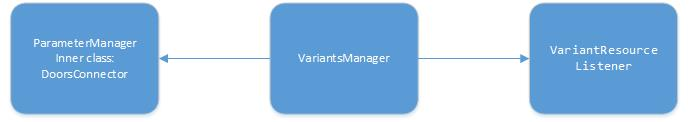
\includegraphics[scale=0.7]{5_1_klassenuebersicht.jpg}
  		  \caption{Darstellung der Klassen}
     \label{ttn.verbindung.klassen.loesung}
  \end{center}
\end{figure}



%#######################################################################################
\subsection{Listener}
Das auslösendes Element ist, dass der Benutzer eine Anforderung mit einen Baumelement verknüpft. Um dieses Geschehen abzufragen wurde ein \textit{Listener} programmiert, der das Interface \textit{ResourceSetListener}\footnote{http://download.eclipse.org/modeling/emf/transaction/javadoc/1.0.3/org/eclipse/emf/transaction/ResourceSetListener.html} implementiert. Die Aufgabe des \textit{ResourceSetListener} ist, dem Benutzer zu benachrichtigen, wenn sich eine Ressource ändert. Der \textit{Listener}  \glqq hört\grqq~ auf die reinkommenden Nachrichten (\textit{ResourceSetChangeEvent}) und wertet den Inhalt dieses Events aus.\\

Als Inhalt der Nachricht wird folgendes empfangen: 

\begin{itemize}
\item \textbf{Event: }ResourceSetChangeEvent, heißt die Ressourcen des Objektes haben sich geändert
\item \textbf{Notifier: } welches Objekt schickt die Nachricht
\item \textbf{Notification: }Beschreibung von der Änderung im \textit{Notifier}
\item \textbf{OldValue: } alter Wert, wenn nicht vorhanden \textit{null}
\item \textbf{NewValue: } neuer Wert, beim löschen von Werten \textit{null}
\end{itemize}

Hier wird als erstes der \textit{Notifier} abgefragt um zu unterscheiden, ob die Nachricht für uns relevant ist. Ist der \textit{Notifier} eine Instanz eines Baumelementes, so wurde eine Anforderung zum ersten mal an das Baumelement verknüpft. \\

Lautet der \textit{Notifier} Instanz von \textit{RequirementTag} so wurde eine Anforderung von einem Baumelement gelöscht oder es wurde eine neue Anforderung an einen Baumelement hinzugefügt, wo schon Anforderung verknüpft waren. Für alle drei Fälle muss der \textit{Listener} wissen:

\begin{itemize}
\item An welches Element wurde das Event ausgelöst?
\item Welche Anforderung wurde hinzugefügt oder gelöscht?
\end{itemize}

Dafür wird aus dem \textit{Notifier} mit der Methode \texttt{getID()} die Identifikationsnummer des zuständiges Baumelement abgefragt. Weiterhin steht im \textit{Notifier} auch die Kennung der Anforderung (diese wurde in DOORS vergeben). Diese beide Informationen werden gespeichert und an den \textit{VariantsManager} weiter gegeben. Diese Informationen sind für der \textit{ParameterManager} nötig, damit er aus der Anforderung die Parameter lesen kann und mit das richtige Baumelement verknüpfen kann.\\




%#######################################################################################
\subsection{VariantsManager}
Die Hauptaufgabe des \textit{VariantsManager} ist die Varianten zu regeln. Hier werden Baumelemente zu  Varianten hinzugefügt und gelöscht. Dabei muss das Klassifikationsbaum neu gezeichnet werden. Diese Klasse kümmert sich auch, um die Umschaltung zwischen Varianten in der Variantenansicht (siehe Abbildung \ref{ttn.generic}). Der \textit{VariantsManager} setzt die Baumelement-ID und die Anforderungskennung in der Klasse \textit{ParameterManager}. Die Klasse dient als Schnittstelle zwischen der \textit{Listener} und die Klasse \textit{ParameterManager}\\

Der \textit{VariantsManager} fragt den \textit{Editor} (beinhaltet das Klassifikationsbaum) nach das benötigte Baumelement über die von \textit{Listener} übergebene Identifikationsnummer. Das Baumelement wird dann in das \textit{ParameterManager} gespeichert. Die Anforderungskennung wird auch im Objekt von \textit{ParameterManager} gespeichert.\\






%#######################################################################################
\subsection{ParameterTag und ParameterTagImpl}\label{sub.ParameterTag}





%#######################################################################################
\subsection{ParameterManager}\label{sub.ParameterManager}

%\begin{figure}[h!]
%  \begin{center}
%    \includegraphics[scale=0.7]{.jpg}
%  		  \caption{Darstellung der Klasse ParameterManager in UML}
%     \label{ttn.ParameterMananger}
%  \end{center}
%\end{figure}

Die Klasse \textit{ParameterManager} beinhaltet eine private innere Klasse \textit{DoorsConnector}(siehe \ref{sub.DoorsConn}), diese kümmert sich um den Verbindungsaufbau mit DOORS.\\ Weiterhin baut die Klasse die vom \textit{Listener} weitergegeben Daten (Baumelement und Anforderungskennung) auf.\\



Anforderung eines Baumelementes beinhaltet Modul und Interface. wichtig für nächstes Kapitel



%#######################################################################################
\subsection{DoorsConnector}\label{sub.DoorsConn}

%\begin{figure}[h!]
%  \begin{center}
%    \includegraphics[scale=0.7]{.jpg}
%  		  \caption{Darstellung der innere Klasse DoorsConnector in UML}
%     \label{ttn.DoorsConnetor}
%  \end{center}
%\end{figure}

Die private innere Klasse \textit{DoorsConnector} baut die Verbindung zwischen den TESTONA und DOORS auf. Sie implementiert das Interface \textit{IConnectionListener}, dass ein \textit{Listener} für die Verbindung-Events umfasst.\\

Als erstes wird von der Klasse \textit{ParameterManager} die Methode \texttt{connectToDoors()} aufgerufen. Diese baut die Verbindung auf, indem gespeicherte Verbindungsdaten aufgerufen werden. Wie bereits in Kapitel \ref{sub.ParameterManager} erwähnt, steht in der Anforderung in welches Modul sich die Anforderung befindet, sowie über welches Interface dieses Modul zu erreichen ist. Für den Verbindungsaufbau werden noch folgende Objekte benötigt:

\begin{itemize}
\item \textbf{DataInterface: }Über diese Klasse erfolgt die Datenanfrage an DOORS. Die Verbindung wird aufgebaut sowie getrennt. Es werden als erstes die Ordner geladen, danach einzelne Projekte und die nötige Module. Es können verschiedene Darstellungen der Module auch geladen werden (diese müssen in DOORS definiert sein). Hier werden auch direkt einzelne Anforderungen angefragt. Relevant für diese Arbeit ist, dass hiermit das Modul Parametertabelle in DOORS geladen wird.
\item \textbf{PreferenceManagment: } Hier werden die in TESTONA gespeicherte Verbindungsdaten behandelt. Es können Microsoft Access Verbindungensdaten gespeichert werden, aber wir werde nur DOORS betrachten.
\item \textbf{Connector: }beschreibt eine einzelne Verbindung, hat ein \textit{DataIterface}- und \textit{PreferenceManagmentobjekt}
\item \textbf{ConnectionManager: }Singleton. Die Klasse handelt aktive und offene Verbindungen. Hier werden die \textit{ConnectionListeners} und das \textit{DataInterface} für den richtigen \textit{Connector} geregelt.
\end{itemize}

Wenn die Verbindung aufgebaut ist, müssen die Ordner und Projekte geöffnet werden bis zur Parametertabelle.....\\

muss programmiert werden\\

Parameter local in Objekt gespeichert\\
Datenmenge relativ gering, deswegen eine Verbindung 

Da die Datenmenge von einer Parametertabelle relativ gering ist, wurde hier, bezüglich der offene Frage bei dem Lösungsansatz (siehe Kapitel \ref{sec.parameterspeicherung}), die Parametertabelle komplett importiert. Es wird angenommen, wenn der Benutzer die Parameterersetzung für ein Parameter wahrnimmt, dass er es für die anderen Parameter auch wahrnehmen wird. Darum wird die Parametertabelle erst bei der Verknüpfung von einer Anforderung mit einem Baumelement importiert, und nicht beim Import der Anforderungen. Weiterhin, um die Rechen- und Reaktionszeit von TESTONA gering zu halten, wird die Tabelle komplett importiert, um nicht für jedes neue Parameter eine Verbindung mit DOORS aufzubauen.


Am ende wird die Verbindung getrennt\\




%#######################################################################################
%#######################################################################################
\newpage
\section{Testfallgenerierung und Optimierung}
\paragraph{}
Erläuterung der Lösungen zu 4.3